\documentclass[tikz,border=5mm]{standalone}
\usepackage{amsmath}
\DeclareMathOperator*{\argmax}{argmax}
\usepackage{amssymb}
\usepackage{bm}
\usetikzlibrary{arrows.meta, positioning, shapes, calc, fit, decorations.pathreplacing}

% Define colors
\definecolor{embColor}{RGB}{252,224,225}
\definecolor{middleColor}{RGB}{220,223,240}
\definecolor{softmaxColor}{RGB}{203,231,207}
\definecolor{tokenColor}{RGB}{240,240,240}
\definecolor{textColor}{RGB}{220,220,220}
\definecolor{boxTextColor}{RGB}{60,60,60}  % Darker text for inside boxes

\begin{document}
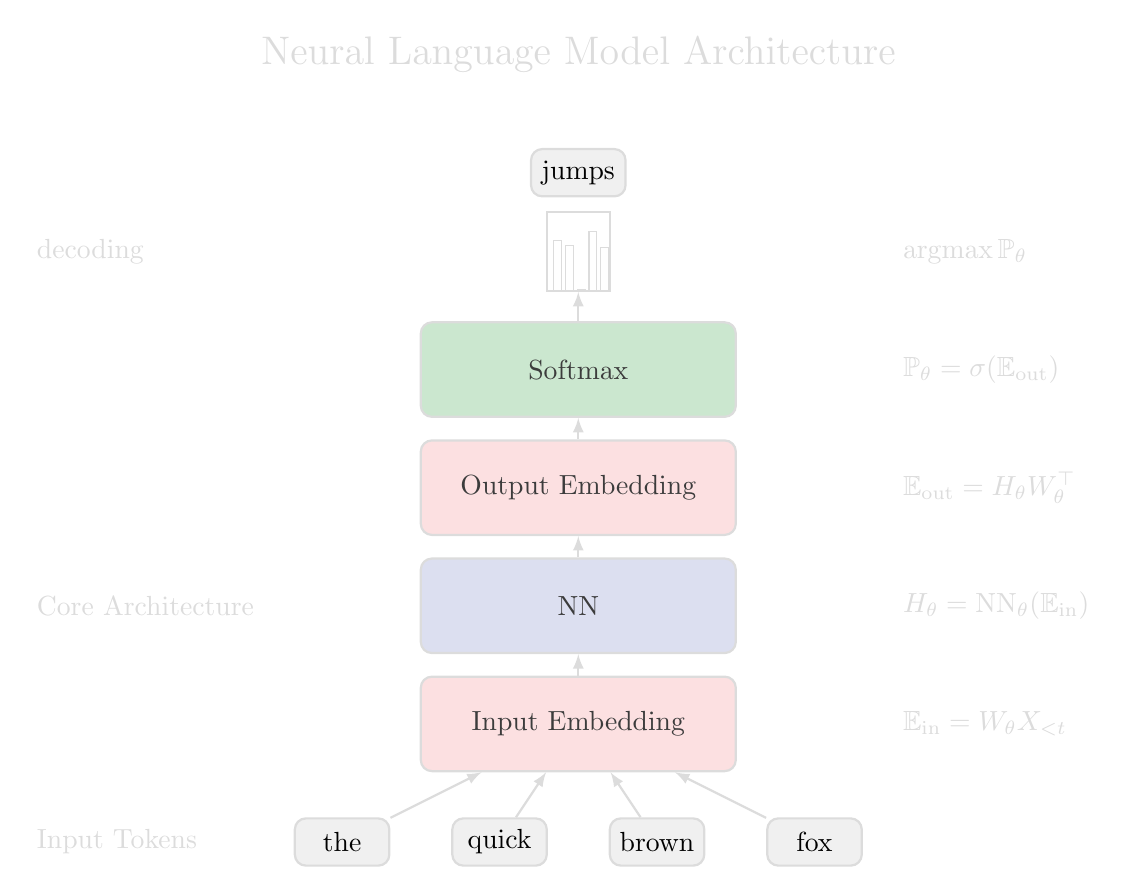
\begin{tikzpicture}[
    box/.style={draw=textColor, thick, minimum width=4cm, minimum height=1.2cm, rounded corners, text=boxTextColor},  % Dark text in boxes
    token/.style={draw=textColor, thick, minimum width=1.2cm, minimum height=0.6cm, fill=tokenColor, text=black, rounded corners},
    dist/.style={draw=textColor, thick, minimum width=0.8cm, minimum height=1cm},
    margin_text/.style={text=textColor, align=left},
    >=latex,
    node distance=1cm,
    every node/.style={text=textColor}
]

% Define column positions
\def\leftmargin{-7cm}
\def\rightmargin{4cm}
\def\diagramwidth{4cm}

% Title centered over the diagram area
\node (title) at (0,7) {\Large Neural Language Model Architecture};

% Output token at top (only "jumps")
\node[token] (t3) at (0,5.5) {jumps};

% Output distribution (only for "jumps")
\node[dist] (d3) at (0,4.5) {};

% Add small bar charts in distribution
\foreach \i in {0,...,4} {
    \draw[textColor] (d3.south west)+(\i*0.15+0.1,0) rectangle +(\i*0.15+0.2,{random()*0.8});
}

% Left and right margin text for distribution
\node[margin_text, right] at (\rightmargin,4.5) {$\argmax \mathbb{P}_\theta$};
\node[margin_text, right] at (\leftmargin,4.5) {decoding};

% Softmax layer
\node[box, fill=softmaxColor] (softmax) at (0,3) {Softmax};
\node[margin_text, right] at (\rightmargin,3) {$\mathbb{P}_\theta = \sigma(\mathbb{E}_\text{out})$};

% Output embedding
\node[box, fill=embColor] (out_emb) at (0,1.5) {Output Embedding};
\node[margin_text, right] at (\rightmargin,1.5) {$\mathbb{E}_{\text{out}} = H_\theta W_\theta^\top$};

% Middle architecture (neural network)
\node[box, fill=middleColor] (middle) at (0,0) {NN};
\node[margin_text, right] at (\rightmargin,0) {$H_\theta = \text{NN}_\theta(\mathbb{E}_\text{in})$};
\node[margin_text, right] at (\leftmargin,0) {Core Architecture};

% Input embedding
\node[box, fill=embColor] (in_emb) at (0,-1.5) {Input Embedding};
\node[margin_text, right] at (\rightmargin,-1.5) {$\mathbb{E}_{\text{in}} = W_\theta X_{<t}$};

% Input tokens
\node[token] (tok1) at (-3,-3) {the};
\node[token] (tok2) at (-1,-3) {quick};
\node[token] (tok3) at (1,-3) {brown};
\node[token] (tok4) at (3,-3) {fox};

% Input Tokens label
\node[margin_text, right] at (\leftmargin,-3) {Input Tokens};

% Connections with light colored arrows
\foreach \i in {1,2,3,4} {
    \draw[->, thick, textColor] (tok\i) -- (in_emb);
}

\draw[->, thick, textColor] (in_emb) -- (middle);
\draw[->, thick, textColor] (middle) -- (out_emb);
\draw[->, thick, textColor] (out_emb) -- (softmax);
\draw[->, thick, textColor] (softmax) -- (d3);

\end{tikzpicture}
\end{document}